\documentclass{report}
\usepackage[utf8]{inputenc}
\usepackage{natbib}
\usepackage[pagestyles]{titlesec}
\usepackage[hidelinks]{hyperref}
\usepackage{pdfpages}
\usepackage{graphicx}
\usepackage{multicol}
\usepackage{multirow}
\usepackage{booktabs}
\usepackage{array}
\usepackage{tabularx}
\usepackage{ltablex}
\newcolumntype{L}[1]{>{\raggedright\arraybackslash}p{#1}}
\newcolumntype{C}[1]{>{\centering\arraybackslash}p{#1}}
\newcolumntype{R}[1]{>{\raggedleft\arraybackslash}p{#1}}


\titleformat{\chapter}[display]{\normalfont\bfseries}{}{0pt}{\Huge}
\newpagestyle{mystyle}
{\sethead[\thepage][][\chaptertitle]{}{}{\thepage}}
\pagestyle{mystyle}

\begin{document}
%TODO: CAMBIARE LA DATA PRIMA DELLA CONSEGNA

\includepdf[pages={1}]{./img/FrontPage}
\tableofcontents
\chapter{Introduction}
This document represents the Requirement Analysis and Specification Document (RASD) for SafeStreets: an application that aims to improve the safety of urban areas by giving its users the possibility to report traffic violations and accidents to authorities. The goal of this document is to supply a description of the system in terms of its functional and non-functional requirements, listing all of its goals, discussing the constraints and the limits of the software, and indicating the typical use cases that will occur after the release. This document is addressed to the stakeholders, who will evaluate the correctness of the assumptions and decisions contained in it, and to the developers who will have to implement the requirements.
\section{Purpose}
SafeStreets is a crowd-sourced application that intends to provide users with the possibility to notify authorities when traffic violations and accidents occur. In order to report a traffic violation, users have to compile a report containing a picture of the violation, the date, time, position, and type of violation. SafeStreets stores all the information provided by users, completing it with suitable metadata (timestamps, sender's GPS if available, etc.). In particular, in case the user had not provided any information regarding the license plate of the car breaking the traffic rules, SafeStreets runs an algorithm to read it from the submitted picture. Moreover, the application allows both end-users and authorities to mine the information that has been received: this function allows users to perform useful statistics, for example to find out which area is more dangerous or which vehicles commit the most violations. If the municipality offers a service that allows users to retrieve the information about the accidents that occur in its territory, SafeStreets can cross this information with its own data to identify potentially unsafe areas, and suggest possible interventions.
In addition, the municipality could offer a service that takes the information about the violations coming from SafeStreets, and generates traffic tickets from it. In this case, SafeStreets ensures that the chain of custody of information coming from users is never broken, thus information is never altered. Information about issued tickets can be used by SafeStreets to build statistics, for example to have a feedback on the effectiveness of the application.
\subsection{Goals}
\begin{itemize}
    \item {[G.1]} The System allows Users to access the functionalities of the application from different locations and devices.
	\item {[G.2]} The System allows Guests to authenticate
	 themselves either as Authority or Citizen.
    \item {[G.3]} The System allows the Citizens to document traffic violations and accidents to Authorities by compiling a Report.
    \item {[G.4]} The System stores the reports provided by the Citizens.
    \begin{itemize}
    		\item {[G.4.1]} If the Citizen has not provided any information about the license plate, the System runs an algorithm to read it from the submitted picture.
		\end{itemize}     
	\item {[G.5]} The System allows Authorities to consult the reports submitted by the Citizens.
    \item {[G.6]} The System analyzes the stored information to detect unsafe areas.
    \begin{itemize}
    		\item {[G.6.1]}If allowed by the Municiplaity, SafeStreets can cross their information about accidents with its own in order to improve the analysis.
	\end{itemize}  
	\item {[G.7]} The System detects unsafe areas through statistics.
	\begin{itemize}
		\item The System can suggest possible interventions to the Authorities.
	\end{itemize}
    \item{[G.8]} If allowed by the Municiplaity, SafeStreets can access their information about issued tickets to build statistics and evaluate its effectiveness.
    \begin{itemize}
        \item {[G.8.1]} The System ensures that the chain of custody of the information coming from the Citizens is never broken.
	\end{itemize}
	\item {[G.9]} The System allows the User to consult statistics
	\begin{itemize}
		\item {[G.9.1]} The System offers different levels of visibility to different roles.
	\end{itemize}
\end{itemize}

\section{Scope}
According to the \textit{World} and \textit{Machine} paradigm, proposed by M. Jackson and P. Zave in 1995, we can distinguish the \textit{Machine}, that is the portion of the system to be developed, from the \textit{World}, that is the portion of the real-world affected by the machine. In this way, we can classify the phenomena in three different types: World, Machine and \textit{Shared} phenomena, where the latter type of phenomena can be controlled by the world and observed by the machine or controlled by the machine and observed by the world.
\newline
In this context, the most relevant phenomena are organized as in the following table.
\clearpage
\begin{table}[!ht]
		%{pix.acc.} & {mean.acc.} & {mean.IoU} & {f.w.IoU}
		\begin{center}
		%\hspace{-4.5cm}
		\begin{tabular}{|C{.28\textwidth}||C{.28\textwidth}||C{.28\textwidth}|}
			\toprule
			\textbf{World} &\textbf{Shared}& \textbf{Machine}\\
			\midrule
			\midrule
			\textbf{Traffic violation}: circumstance in which someone doesn't respect the traffic rules &\textbf{\small{Registration/Login}}$^{1}$: a Guest can sign up to the application or log in if already registered.&\textbf{DBMS query}: operation performed to retrieve/store data\\
			\midrule
			\textbf{Accident}: event that caused damage to things or people.&\textbf{Commit of a report}$^{1}$: action of sending a report documenting a traffic violation or an accident.&\textbf{API queries}: request for third-part services.\\
			\midrule
			&\textbf{Send notifications}$^{2}$: to notify the Autorithies when a report is submitted.&\textbf{Encrypt data}: to compute the hash function to ensure that reports are never altered and that user's credentials are safe.\\
			\midrule
			&\textbf{Build statistics}$^{2}$: computation of statistics to find unsafe areas, to see which veichles commit multiple infractions and also to monitor the trend of issued tickets.&\textbf{Role Isolation}: to grant different levels of visibility to Citizen and Authorities\\ 
			\midrule			
			&\textbf{Safety suggestions}$^{2}$: to give suggestions for possible safe interventions (e.g add a barrier).&\\
			\bottomrule
		\end{tabular}
		\end{center}
		\caption{In the table above, \textit{1} refers to shared phenomena controlled by the world and observed by the machine, whereas \textit{2} refers to the phenomena controlled by the machine and observed by the world}.
		\label{tab:multicol}
	\end{table}

\section{Definitions, Acronyms and Abbreviations}
\subsection{Definitions}
\begin{itemize}
	\item \textit{System}: the totality of the hardware/software applications that contribute to provide the service concerned.
    \item \textit{Guest}: someone who has yet to sign up and who is not able to access any feature of the application.
    \item \textit{User}: a registered user who has logged in.
	\begin{itemize}
		\item \textit{Citizen}: end-user who can send Reports of traffic violation. It has limited visibility over the stored information.
		\item \textit{Authority}: user who has access to the history of Reports and is notified whenever a new Report is recieved. It has full visibility over the data exposed by the System.
	\end{itemize} 
	\item \textit{Municipality}: a single administrative division with its own local government. It stores sensitive information about the Authorities and their work (g.e. traffic tickets).
    \item \textit{Traffic violation}: occurrence of drivers that violate laws that regulate vehicle operation on streets and highways(e.g double-way parking).
    \item \textit{Report}: documentation of a traffic violation. It contains a picture of the violation, the date, time, position, and type of violation. Some fields can be omitted in case an accident is being reported.
    \item \textit{Hash}: a mathematical algorithm that maps data of arbitrary size to a bit string of fixed size. It is a one-way function, that is, a function which is practically infeasible to invert.
    \item \textit{Chain of custody}: chronological documentation that records the sequence of custody, control, transfer, analysis, and disposition of physical or electronic evidence.
    \item \textit{Third-party services}: services used by the System in order to provide extra functionalities (e.g. image recognition).
    %\item \textit{Notification}: message that advise the Authorities of a traffic violation.
\end{itemize}
\subsection{Acronyms}
\begin{itemize}
\item \textbf{API}: \textit{Application Program Interface}, set of routines, protocols and tools for building software applications on top of this one.
\item \textbf{OCR}: \textit{Optical Character Recognition}, software dedicated to the detection of characters contained in a document and to their transfer to digital text that can be read by a machine. In this context, OCR will be used to read license plates.
\item \textbf{UML}: \textit{Unified Modeling Language}, is a standard visual modeling language intended to be used for analysis, design, and implementation of software-based systems.
\item \textbf{GPS}: \textit{Global Positioning System}, technology widely used to get the user's position.
\item \textbf{DBMS}: \textit{Data Base Management System}, software that provides organized space memory to store information.
\item \textbf{ID}: \textit{Identification}, a unique key given to each registered User.
\end{itemize}
\subsection{Abbreviations}
\begin{itemize}
\item {[G$_{i}$]}: i-th goal.
\item {[R$_{i}$]}: i-th requirement.
\item {[D$_{i}$]}: i-th domain assumption.
\end{itemize}
\section{Reference Documents} \label{docs}
\begin{itemize}
	\item Specification document: \textit{SafeStreets Mandatory Project Assignment.pdf}.
	\item IEEE std 830-1998:  \href{http://www.math.uaa.alaska.edu/~afkjm/cs401/}{\textit{IEEE Recommended Practice for Software Requirements Specifications}}.
	\item ISO/IEC 9126-1:2001: \href{https://www.iso.org/standard/22749.html}{\textit{Software engineering — Product quality — Part 1: Quality model}}
	\item Alloy docs: \url{http://alloy.lcs.mit.edu/alloy/documentation.html}.
	\item UML diagrams: \url{https://www.uml-diagrams.org}.
\end{itemize}
\section{Document Structure}
This document is presented as it follows:
\begin{enumerate}
	\item {\textbf{Introduction}} contains a general description of the system and its goals, presenting the problem in an informal way.
	\item{\textbf{Overall description}} gives a general description of the application, focusing on the context of the system and giving further details about shared phenomena. Furthermore, we will provide the specifications of constraints, dependencies and assumptions, that show how the System is integrated with the real world.
	\item{\textbf{Specific requirements}} goes into details about functional and non-functional requirements and a list of all possible interctions with the System is provided using use cases and sequence diagrams.
	\item {\textbf{Formal analysis using Alloy}} contains the Alloy model of some critical aspects of the System with all the related comments. A proof of consistency and an example of the generated world are also provided.
	\item {\textbf{Effort spent}} shows the time spent writing this document by each member of the team.
	\item {\textbf{References}}
\end{enumerate}

\chapter{Overall Description}
\section{Product Perspective}
We are going to analyze all the shared phenomena that are listed in the previous section. The concepts are clarified through class and state diagrams.\\ \vspace{2mm}

\noindent\textbf{Registration/Login} (World controlled, Machine observed)\\
A Guest can sign up to the application or log in, if already registered. 
In the case of a new submit, the System provides a form which the Guest have to fill with his data, specifying if he/she is 
a Citizien or an Authority.\\ \vspace{2mm}

\noindent\textbf{Commit of a report} (world controlled, machine observed)\\
A Citizen can send a Report with a description of the violation compiling a structured field. He/she has the possibility to  attach a picture. The System will check if the compiled fields are consistent and complete, then it will encrypt the Report and send it to the DBMS (Figure \ref{fig:State1}). \\ \vspace{2mm}

\noindent\textbf{Send Notification} (Machine controlled, World observed)\\
The System notifies the Authorities whenever a new Report is submitted by a Citizen. 
We assume that the notified Authorities will accordingly handle the violation reported. (Figure \ref{fig:State1}).
\begin{figure}[!ht]
\begin{center}
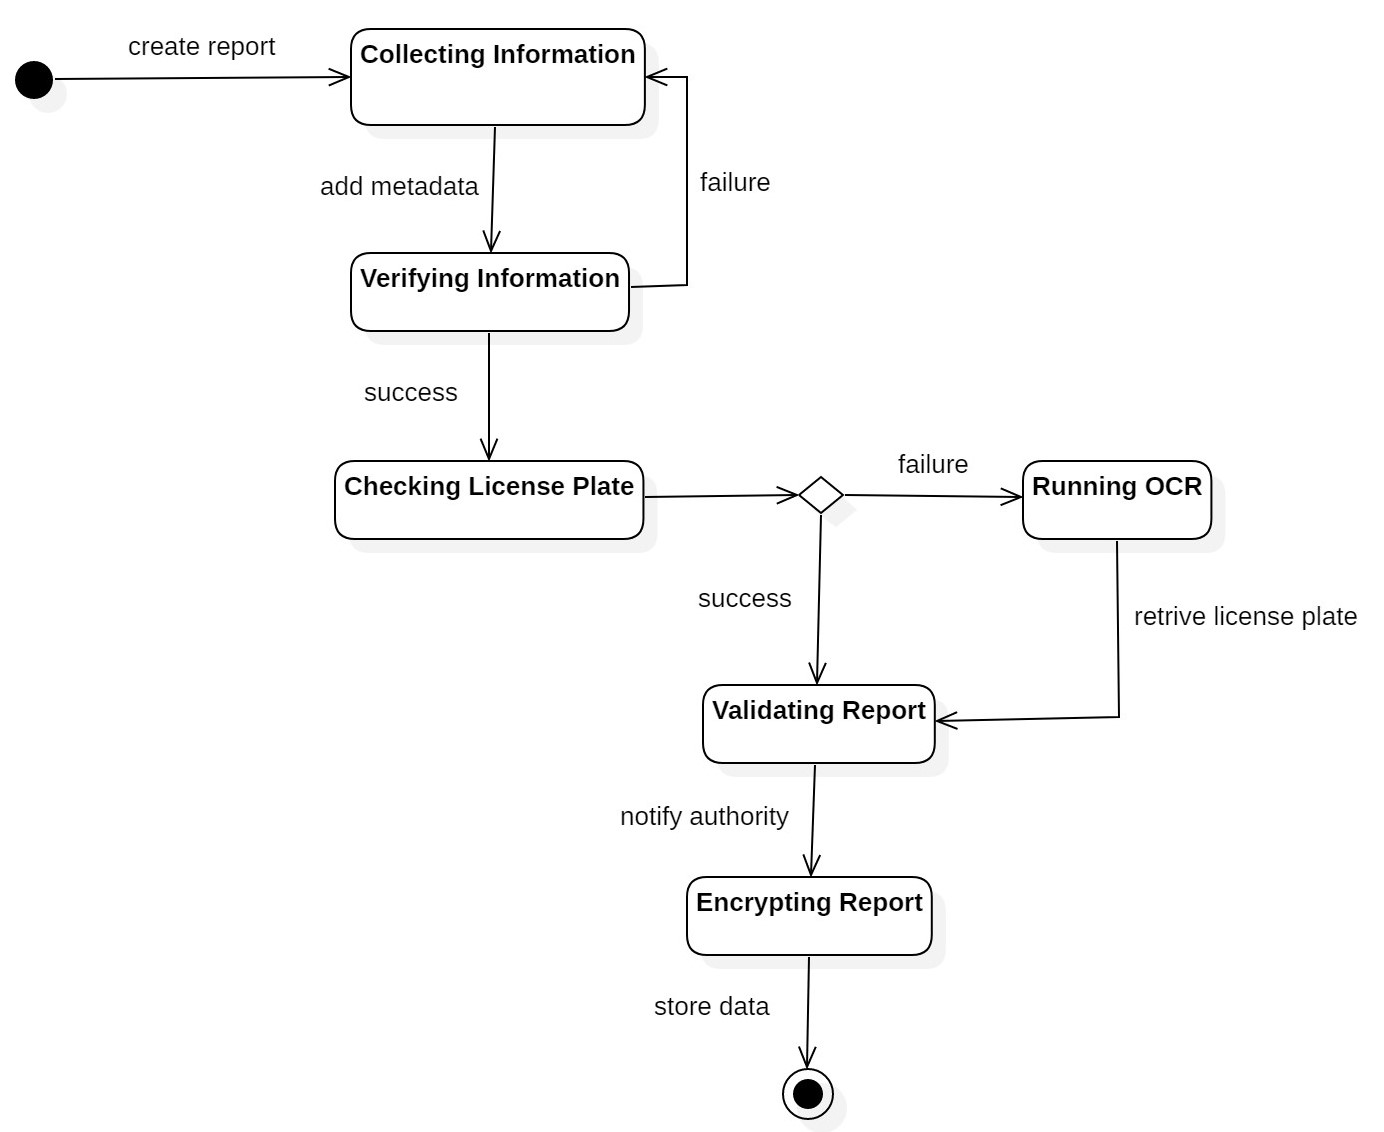
\includegraphics[width=.8\textwidth]{./img/Statechart_Report.jpg}
\end{center}
\caption{SafeStreets' statechart diagram about the collection, notification, and storage of a Report.}
\label{fig:State1}
\end{figure} 
\newpage
\noindent\textbf{Build statistics} (Machine controlled, World observed)\\
The System analyzes the stored data and computes general statistics on the violations. In this way, the System is able to find unsafe areas and which vehicles commit the most violations. All Users can access general statistics, however only Authorities can request statistics on private information such as traffic tickets. If the System is allowed to access Municipality's data, statistics can be enhanced by crossing it with SafeStreets' information (Figure \ref{fig:State2}).  \\ \vspace{2mm}

\noindent\textbf{Safety suggestions} (Machine controlled, World observed)\\
The System gives Authorities suggestions for possible safe interventions. His knowledge is based on the statistics previously computed (Figure \ref{fig:State2}).

\begin{figure}[!ht]
\begin{center}
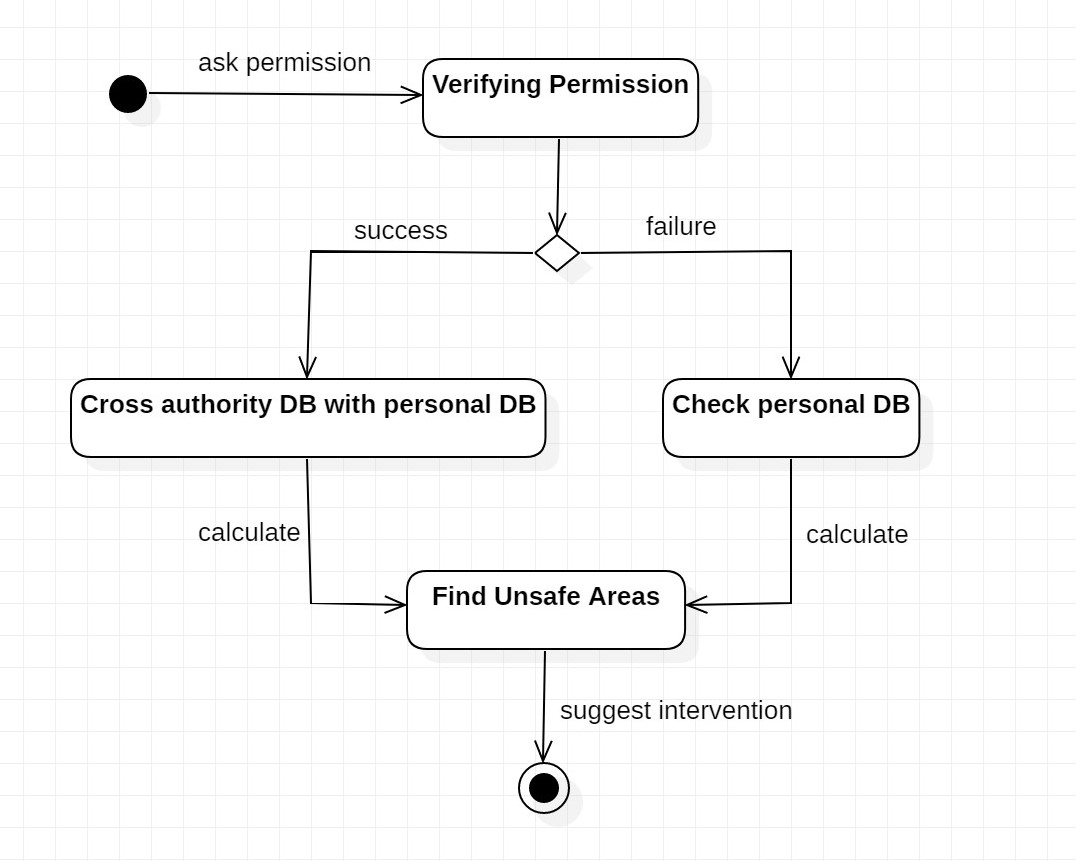
\includegraphics[width=.8\textwidth]{./img/img_UnsafeAreas.jpg}
\end{center}
\caption{SafeStreets' statechart diagram of the creation of statistics on unsafe areas.}
\label{fig:State2}
\end{figure}
\newpage
\subsection{Class Diagram}
The class diagram in Figure \ref{fig:UML} shows a possible representation of the Safe Streets' architecture. Notice that the Municipality's DBMS is only accessible by the System if SafeStreets is authorized by the AccessController. It's also important to outline that the System is not designed to provide a function to generate official traffic tickets, since only real world authorities (g.e. local police) can generate traffic tickets with legal validity.
\begin{figure}[!ht]
\begin{center}
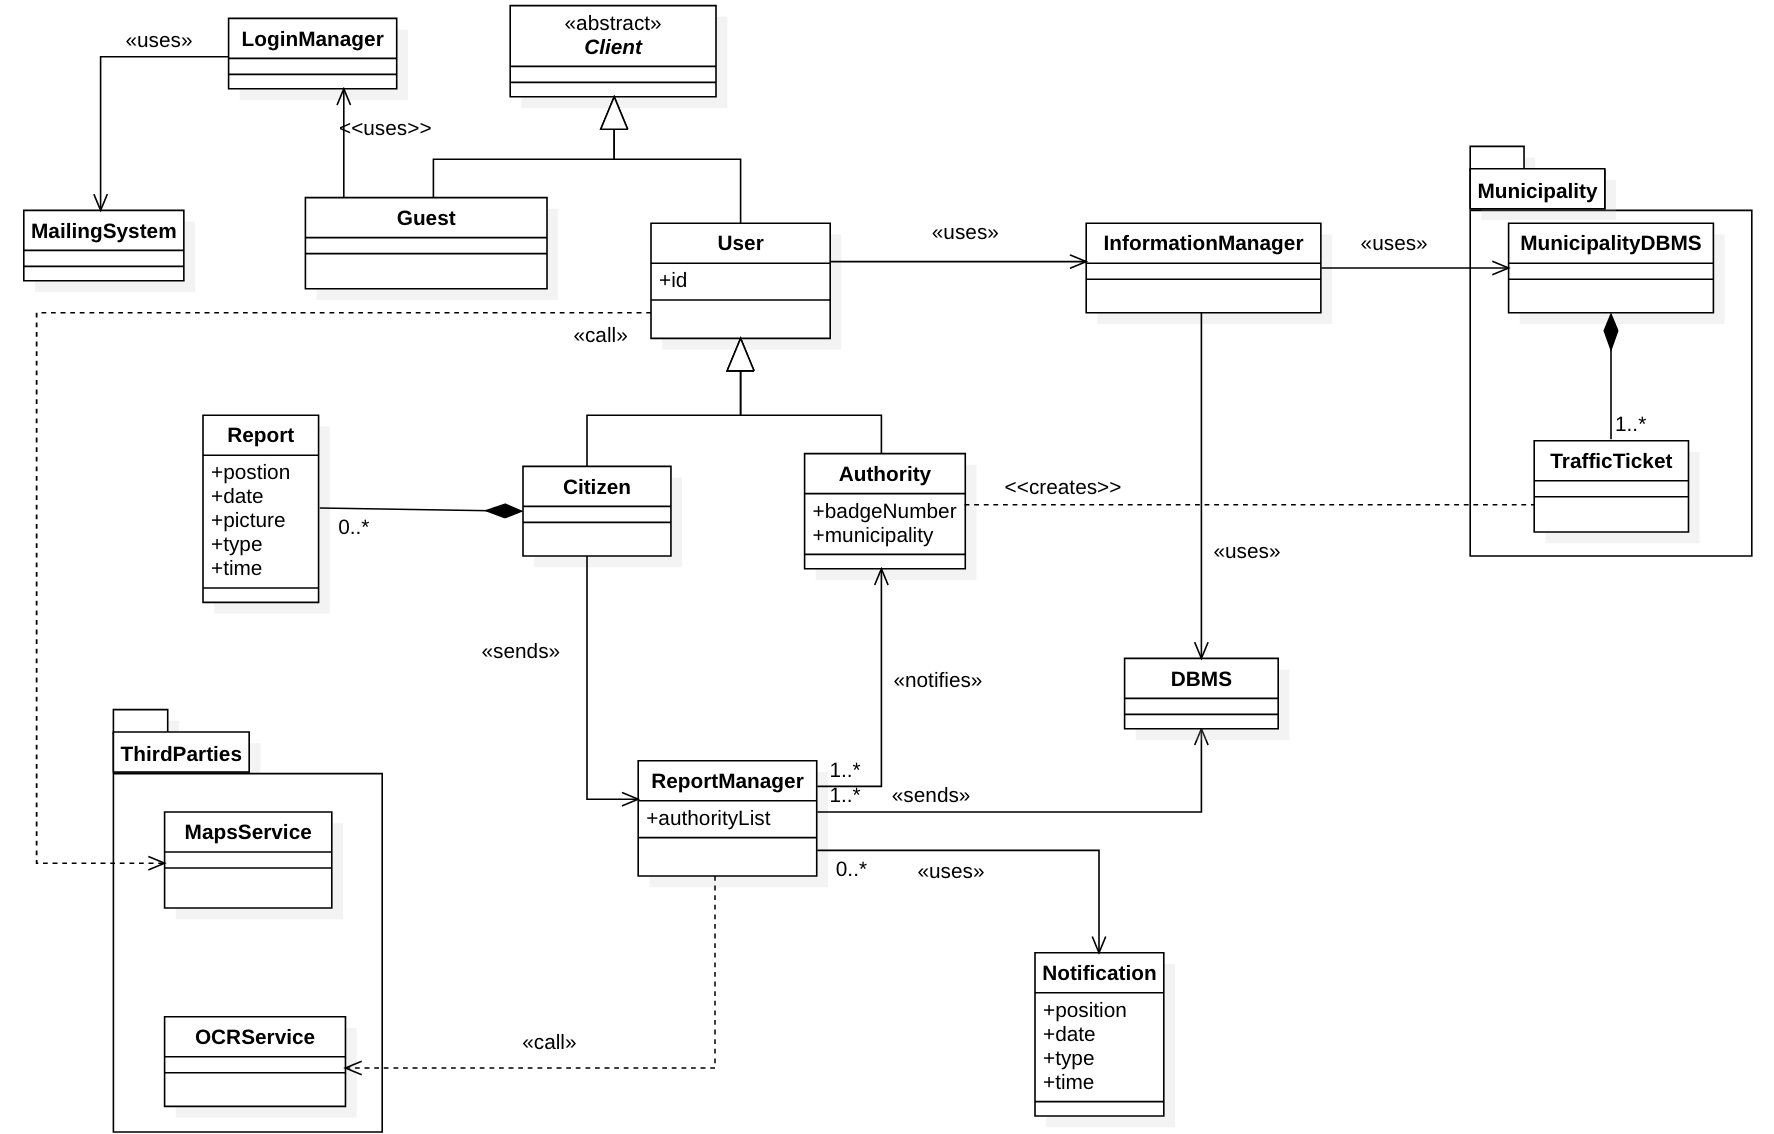
\includegraphics[width=\textwidth]{./img/SWE1.png}
\end{center}
\caption{SafeStreets' class diagram.}
\label{fig:UML}
\end{figure} 
\newpage

\section{Product Functions}
In this section the most important features of the application are extensively explained:
\begin{itemize}
	\item \textbf{Commit of a Report}: the System allows a Citizen to notify Authorities whenever a traffic violations occur. This function is achieved by compiling a Report with a picture of the violation, the date, time, position, and type of violation. Not all of these fields are always compulsory: for example, in the case the type of violation is \textit{accident}, only date, time and position are required. Once all the information is gathered and the report is sent to SafeStreets, the Report Manager goes in the \texttt{Verifying Information} status: it checks if all the obligatory fields have been compiled correctly, and then adds some useful metadata to the Report. Among the additional metadata, the systems takes note of whether or not the position has been provided by GPS, and also if the sender has added any license plate in the \texttt{Checking License Plate} status. If no license plate has been inserted, the Report Manager runs an OCR algorithm to retrive it from the picture provided (\texttt{Running OCR} status). \\
	After all the steps above, the Report is validated (\texttt{Validating Report} status) and a copy of it is notified to the Authorities, which we assume are going to handle it properly (g.e. dispatching a local police patrol). It is important to outline that the System is only designed to inform Authorities whenever a new report is confirmed, but by no means it provides a function which generates official traffic tickets or dispatches patrols in case of accidents. Also, it's relevant to notice that the Report Manager contains a list of all the Authorities, so it can notify all and only those Authorities who are on duty in the involved municipality. Finally, the Report is encrypted by means of a hash function (\texttt{Encrypting Report} status), thus no one can alter the information after its confirmation (see Section \ref{sec:security} for more details on security). \\
	Once the Report has been validated and encrypted the System is ready to store it: the Report is saved into a local buffer and there awaits to be exported into SafeStreets' database. Each day at a set time (g.e. between day/night shifts of the police) the System permanently stores all the Reports into the database. This mechanism takes advantages of the fact that one does not need fresh data to do general statistics, and in return it gives the possibility to schedule the Report storage when the System is not busy.

	\item \textbf{Build statistics}: the System analyzes the stored data to compute general statistics and returns useful information to the Users. This function is carried out by an Information Manager, which is in charge of retrieving, decrypting and elaborating the information stored by the Report Manager. In particular, the Information Manager periodically executes the following functions:
	\begin{enumerate}
		\item Compute a statistic which highlights the areas and vehicles with the highest frequency of violations.
		\item \label{func2} Identify potentially unsafe areas by analyzing Reports of accidents, and suggest possible interventions.
		\item \label{func3} Analyze traffic ticket trends to build statistics about the most recurrent offenders and the effectiveness of SafeStreets.
	\end{enumerate}
	Every User can request to see the latest result of the functions above as soon as they are available. Since both Citizen and Authorities have access to those results, it's really important to give them different levels of visibility, so that classified information doesn't end up in the hands of civilians (g.e vehicles with the highest frequency of violations and most recurrent offenders). It is also worth noting that some of the above functions are enhanced, or even enabled, only if the Municipality grants the Information Manager access to their database. In particular, the Function \ref{func2} can be enhanced by crossing Authorities' accident information with SafeStreets', whereas Function \ref{func3} is entirely enabled only if the System has access to traffic tickets data.

	\item \textbf{Safety suggestions}: the System is able to give Authorities suggestions to improve the safety of urban areas. This function is enabled by the Information Manager and the statistics previously built. In fact, observing for each area which kind of violations are more frequent and the trends of the accidents, the Information Manager runs an artificial intelligence to detect which solution is the most suitable for a given problem. Just like for the report storing process, these suggestions are updated when the System is less busy (g.e. at night) and a sufficient amount of fresh data is added to the database. Safety suggestions are downloaded by SafeStreets' application togeter with the latest statistics results, whenever they are requested. Despite this, it should be noted that only Authorities have access to such data, as they are assumed to be those who implement the suggestions in order to improve their service.
\end{itemize}

\section{User Characteristics}
SafeStreets can be used from both Citizens and Authorities. It is recommended for adult users, but there are no limitation of age. 
We take for granted that the Users have access to Internet and are able to install and use the mobile application.\\
The character are:
\begin{itemize}
	\item \textit{Guest}: anyone who downloads and opens the app but still has to sign
	up or log in. He/she cannot use any of the functions provided by SafeStreets.
	\item \textit{User}: a registered Guest who has to logged either as Citizen or as Authority. He/She is recognized by the System through an ID and can access any feature of the application granted for his/her role.
	\item \textit{Citizen}: someone who has logged-in with his credentials, which is recognized by the System through an ID. He/she can access to the personal data menu and add new reports.
	\item \textit{Authority}: someone who has logged-in with his credentials. He/she is notified every time a new Report regarding its municipality is stored by the System.
\end{itemize}

\section{Assumptions, Dependencies and Constraints}
\subsection{Assumptions}
\begin{itemize}
	\item {[D.1]} The registration mail is assumed to be correctly recieved by the User.
	\item {[D.2]} The System internal clock time used to provide notifications is
	correct.
	\item {[D.3]} The Authorities notifications are assumed to be made only in case of parking violations. Indeed, if a little accident occurs there is no need to contact the Authorities. Instead if a dangerous accident happens it is better to call the Autorithies for a promptly intervention. The System uses accident report only to make statistics.
	\item {[D.4]} The Authorities are assumed to  take measures when they are notified about a new report.
	\item {[D.5]} After the first time, the System does not need to request the access to the Municipality's’ DBMS as long as the permission is still valid.
	\item {[D.6]} The statistics and suggestions are assumed to be consulted by Authorities periodically, in order to provide a better service.
	\item {[D.7]} Only specific component of the System is able to decrypt sensible data.
	\item {[D.8]} SafeStreets is not responsible of the traffic tickets generated by Authorities.
\end{itemize}
\subsection{Dependencies}
\begin{itemize}
	\item The System needs a DBMS in order to store and retrieve Users’ Reports.
	\item Information on issued tickets are provided by the Authorities' DBMS, which has limited access. 
	\item The OCR tool is provided by external thrid party services.
	\item The Map service is provided by external an third party (which can be different by the one that provides the OCR) tool.
\end{itemize}
\subsection{Constraints} \label{constraints}
\begin{itemize}
	\item Users must have a smartphone equipped with an OS compatible with the application.
	\item Users must have a working Internet connection.
	\item The System must ask Users for the permission to acquire and store personal data. Therefore, the System must offer the possibility to the Users to delete their personal account.
	\item The System provides statistics on issued tickets but it is not able to acknowledge if the tickets are generated thanks to its service, or if they are independent from Safestreets.
	
\end{itemize}

\chapter{Specific Requirements}
\section{External Interface Requirement}
SafeStreets is a mobile based application. In the following sections a more detailed description of the application is given in terms of hardware, software and communication interfaces. There are also present some prototypes of User Interface through mockups.
\subsection{User Interface}
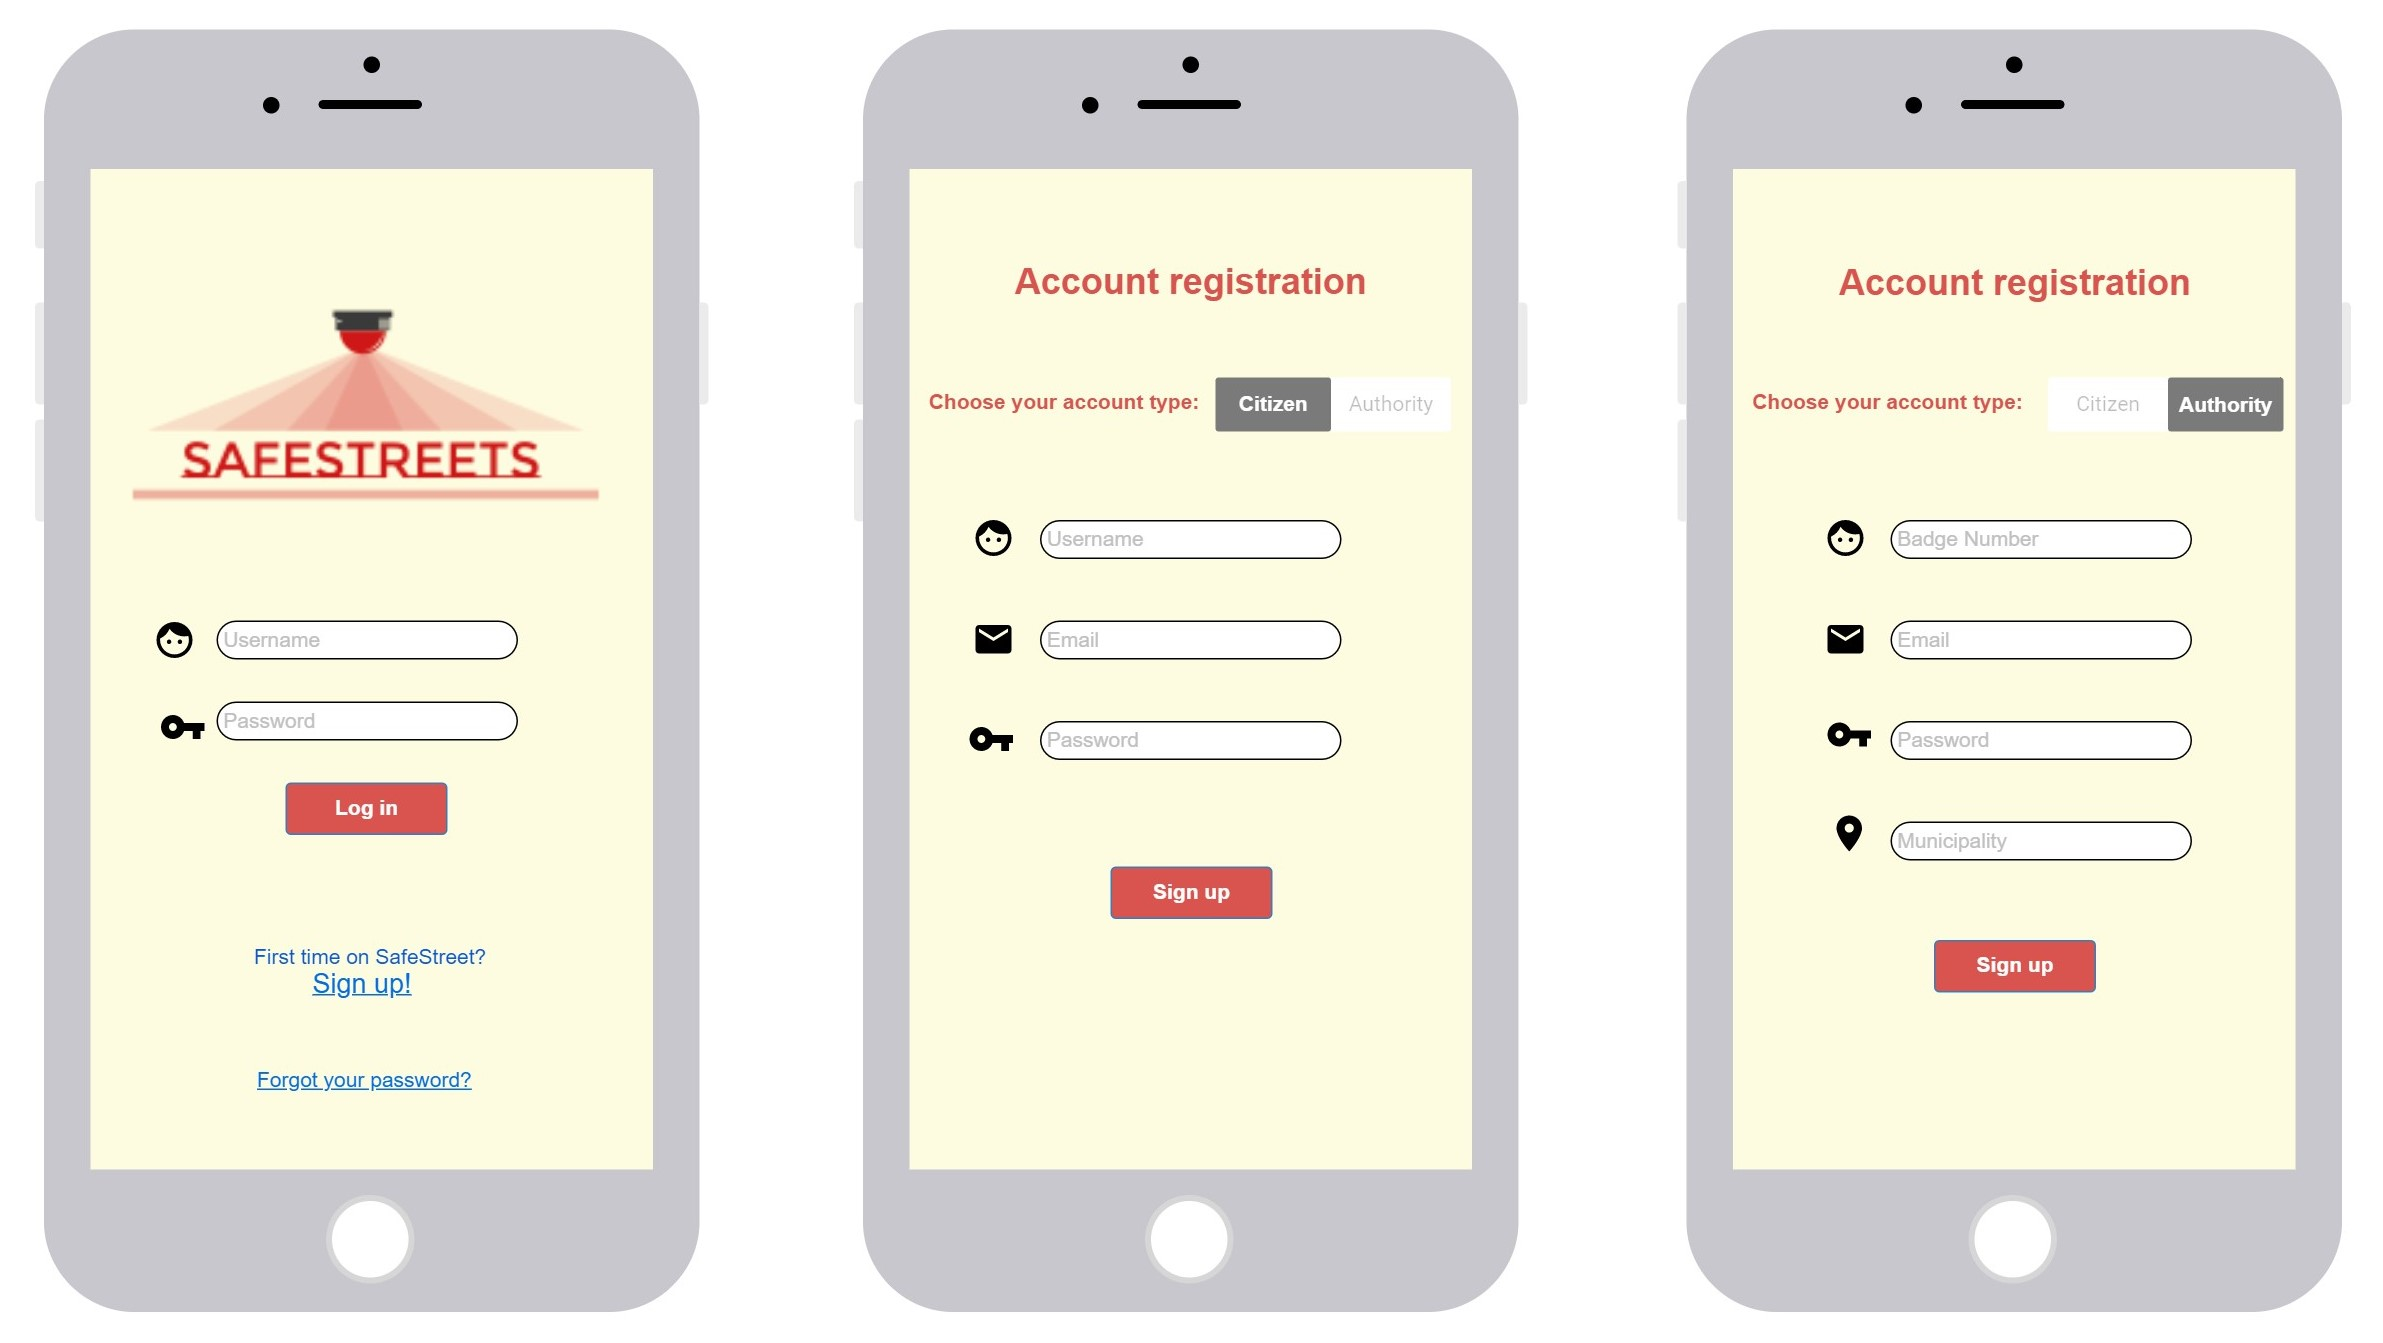
\includegraphics[width=\textwidth]{img/Mockup_logging.jpg}
\subsection{Hardware Interface}
The application is avaiable for mobile devices that guarantee Internet access with a reasonably recent browser and have a camera with a fairly high definition.
\subsection{Software Interface}
\begin{itemize}
\item \textbf{Operating System}: iOS, Android.
\item Web browser.
\item Web Server application.
\item DBMS.
\item \textbf{Report System}: use third part services as OCR.
\item \textbf{Mailing System}: APIs to send emails to the User.
\item \textbf{Mapping System}: APIs to locate the position of the traffic violation.
\end{itemize}
\subsection{Communication Interface}
The application runs over HTTPS protocol for the communication over the Internet and with the DBMS.
\section{Functional Requirements}
In the following section are explained the functional requirements of the application.
\begin{itemize}
	\item {[R.1]} A visitor must be able to register. During the registration the System will ask to provide some credentials.
	\item {[R.2]} The System must check if the Guest credentials are valid:
		\begin{itemize}
			\item the username is not already taken by another registered User.
			\item the email is in the right format.
			\item the password has a minimum length.
			\item the municipality, if it is an Authority.
		\end{itemize}
		If credentials are correct, the System sends a confirmation email.
	\item {[R.3]} The System must store all User data such as personal information and credentials.
	\item {[R.4]} The System must allow the User to log in using his/her personal
	credentials.
	\item {[R.5]} The System must allow the User to change username, only if the
	new username is not already in use by another User, email, only if the
	new email is in a correct format and password, only if the new password
	is different from the precedent and respects the minimum length.
	\item {[R.6]} The System must send a confirmation email if username, email
	or password is changed (similarly to the registration process). 
	\item {[R.7]} The System must allow the User to change password if it has been forgotten, 
	through the personal email.
	\item {[R.8]} The User must be allowed to create reports, specifying:
		\begin{itemize}
			\item The type of report (violation/accident).
			\item The location of the violation/accident.
			\item The date of the violation/accident.
			\item The time of the violation/accident.
			\item A picture of the violation/accident (not mandatory).
		\end{itemize}
	\item {[R.9]} The System must check if the Report created by the User is correct.
	\item {[R.10]} The System must notify the Authorities whenever a new Report involving their municipality is submitted. 
	\item {[R.11]} The System must provide two different level of visibility regarding the statistics. Only the Authorities can consult statistics with private data.
	\item {[R.12]} The System must allow the User to consult the statistics.
	\item {[R.13]} The System provides a recognition system of badge number.
	\item {[R.14]} The System must allow the Citizen to consult the history of its personal reports.
	\item {[R.15]} The System must allow the User to see its position in a map.
	\item {[R.16]} The System notify a copy of a report about traffic violation to Authorities.
	\item {[R.17]} The System provides a list of the most recent reports submitted to the Authorities.
	\item {[R.18]} The System provides an history of reports submitted to the Authorities.
	\item {[R.19]} The System must interact with the Municipality to get the permission for using their data.
	\item {[R.20]} The System can use third party services to enable some of its functions.
	\item {[R.21]} The System has to update the statistics periodically.
	\item {[R.22]} The System must provide protection of data using encryption.
	\item {[R.23]} The System must be able to acknowledge whether or not multiple istances of Reports are referred to the same infraction, even if protracted over time.
	\item {[R.24]} The System can cross the data coming from external DBMS with its own data.
\end{itemize}

\newpage

\subsection{Use Cases}

\begin{figure}[ht!]
\begin{center}
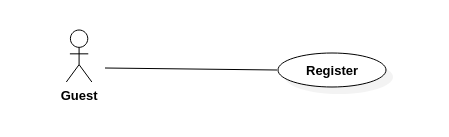
\includegraphics[width=\textwidth]{./img/UseCase1.png}
\end{center}
\caption{Guest use case.}
\label{fig:UseCase1}
\end{figure}
%%%%%%%%%%%%%%%%%%%%%%%%%%%%%%%%%%%%%%%%%%%%%%%%%%%%%%%
\begin{center}
	\textbf{Register Account}
\end{center}

\begin{tabularx}{\linewidth}{| l | X |}
	\hline
	\textbf{ID} & UC1\\
	
	\hline
	\textbf{Description} & The \textbf{\textit{Guest}} wants to create an account for the application.\\
	
	\hline
	\textbf{Actors} & \textbf{\textit{Guest}}, \textbf{\textit{Login Manager}} and \textbf{\textit{Mailing System}}\\
	
	\hline
	\textbf{Preconditions} & The \textbf{\textit{Guest}} downloads and opens the application.\\
	
	\hline
	\textbf{Flow of Events} & \parbox{0.7\textwidth}{	
		\begin{enumerate}
			\item The \textbf{\textit{Guest}} taps the Sign Up button and and selects a role between Citizen or Authority.
			\item Based on the the \textbf{\textit{Guests'}} decision, the \textbf{\textit{Login Manager}} provides the appropriate form to enter all the required data: username, email address and password. In the Authoritys' form the username corresponds to the badge number, and the municipality of belonging must be inserted as well. 
			\item The \textbf{\textit{Guest}} fills the form with all the required information and then confirms the entries. The same procedure will be used for future logins.
			\begin{itemize}
				\item If the \textbf{\textit{Guest}} is an Authority, he/she has to insert his/her badge number as username and provide the municipality of belonging.
			\end{itemize}	
			\item The \textbf{\textit{Login Manager}} checks if all the informa-
			tions are correct, in which case it generates a random activation
			URL and asks the \textbf{\textit{Mailing System}} to forward the URL to the email address of the \textbf{\textit{Guest}}.
			\item The \textbf{\textit{Guest}} receives the mail and clicks on the URL. \item The \textbf{\textit{Login Manager}} accepts the registration and stores the data provided by the \textbf{\textit{User}} .
	\end{enumerate}}\\
	
	\hline
	\textbf{Postconditions} & The \textbf{\textit{Guest}} is now able to log in.\\
	
	\hline
	\textbf{Exceptions} & \parbox{0.7\textwidth}{ \begin{enumerate}
			\item The \textbf{\textit{Login Manager}} realizes that invalid cerdentials have been entered (g.e. the account already exists) and shows an error message. The flow restarts from point 2. 
		\end{enumerate}}\\

	\hline
	
\end{tabularx}

%%%%%%%%%%%%%%%%%%%%%%%%%%%%%%%%%%%%%%

\begin{center}
	\textbf{Log in}
\end{center}

\begin{tabularx}{\linewidth}{| l | X |}
	\hline
	\textbf{ID} & UC2\\
	
	\hline
	\textbf{Description} & The \textbf{\textit{Guest}} wants to log in to the application.\\
	
	\hline
	\textbf{Actors} & \textbf{\textit{Guest}} and \textbf{\textit{Login Manager}} \\
	
	\hline
	\textbf{Preconditions} & A \textbf{\textit{Guest}} wants to log in to the application and is already registered.\\
	
	\hline
	\textbf{Flow of Events} & \parbox{0.7\textwidth}{
		\begin{enumerate}
			\item The \textbf{\textit{Guest}} opens the application and inserts his/her credentials (username and password).
			\begin{itemize}
				\item If the \textbf{\textit{Guest}} is an Authority, he/she has to insert his/her badge number as username.
			\end{itemize}
			\item The \textbf{\textit{Guest}} taps the Log In button.			
			\item The \textbf{\textit{Login Manager}} checks if all the credentials provided are correct.
	\end{enumerate}}\\
	
	\hline
	\textbf{Postconditions} & The \textbf{\textit{User}} is logged in either as Citizen or Authority.\\
	
	\hline
	\textbf{Exceptions} & \parbox{0.7\textwidth}{ 
		\begin{enumerate}
			\item The \textbf{\textit{Login Manager}} recognizes invalid credentials than shows an error message. The flow restarts from point 1. 
		\end{enumerate}}\\
	
	\hline
\end{tabularx}
%%%%%%%%%%%%%%%%%%%%%%%%%%%%%%%%%%%%%%%%%%%%%%%%%%
\begin{figure}[ht!]
\begin{center}
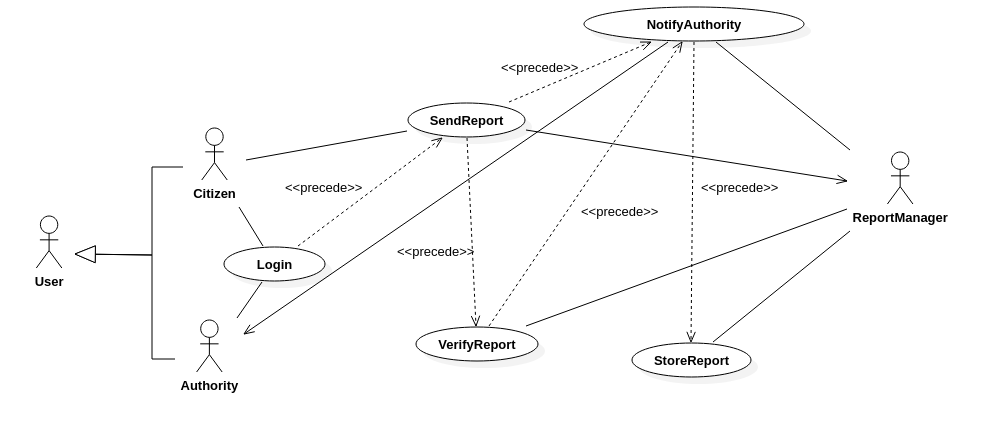
\includegraphics[width=\textwidth]{./img/UseCase2.png}
\end{center}
\caption{User and Report Manager use case.}
\label{fig:UseCase2}
\end{figure}

\begin{center}
	\textbf{Send report}
\end{center}

\begin{tabularx}{\linewidth}{| l | X |}
	\hline
	\textbf{ID} & UC3\\
	
	\hline
	\textbf{Description} & A \textbf{\textit{Citizen}} reports a traffic violation.\\
	
	\hline
	\textbf{Actors} & \textbf{\textit{Citizen}} and \textbf{\textit{Report Manager}}\\
	
	\hline
	\textbf{Preconditions} & The \textbf{\textit{Citizen}} witnesses a traffic violation and wants to report it.\\
	
	\hline
	\textbf{Flow of Events} & \parbox{0.7\textwidth}{\begin{enumerate}
			\item The \textbf{\textit{Citizen}} logs in to the application.
			\item The \textbf{\textit{Citizen}} taps on \textit{Report} button.
			\item The \textbf{\textit{Citizen}} compiles a Report.
			\begin{itemize}
				\item He/She takes a picture of the violation, if possible.
				\item He/She also enters the date, time, location and the type of the violation.			
			\end{itemize}
			\item The \textbf{\textit{Citizen}} taps the \textit{Send} button.
			\item The \textbf{\textit{Report Manager}} checks if the report has been correctly compiled.		
	\end{enumerate}}\\
	
	\hline
	\textbf{Postconditions} & The report is sent and the \textbf{\textit{Citizen}} recives a message that confirms the sending was successfull.\\
	
	\hline
	\textbf{Exceptions} & \parbox{0.7\textwidth}{ \begin{enumerate}
			\item The \textbf{\textit{Report Manager}} rejects the report and shows an error message saying what fields are wrongly compiled. The flow restarts from point 2. 
		\end{enumerate}}\\
	
	\hline
	
\end{tabularx}
%%%%%%%%%%%%%%%%%%%%%%%%%%%%%%%%%%%%%%%%%%%%%%%%%
\begin{center}
	\textbf{Store and Notify report}
\end{center}

\begin{tabularx}{\linewidth}{| l | X |}
	\hline
	\textbf{ID} & UC4\\
	
	\hline
	\textbf{Description} & The \textbf{\textit{Report Manager}} recieves a report from a Citizen and notifies the Authorities about it. Then the report is stored in a database.\\
	
	\hline
	\textbf{Actors} & \textbf{\textit{Report Manager}}\\
	
	\hline
	\textbf{Preconditions} & The \textbf{\textit{Report Manager}} recives a valid report (see UC3).\\
	
	\hline
	\textbf{Flow of Events} & \parbox{0.7\textwidth}{\begin{enumerate}
			\item The \textbf{\textit{Report Manager}} computes metadata (g.e. whether or not license plate has been entered, if position has been provided by GPS, etc.) and attaches them to the Report.
			\item The \textbf{\textit{Report Manager}} runs an API call to retrieve any information about the license plate by means of an external OCR.
			\item The \textbf{\textit{Report Manager}} notifies the Authorities of the municipality where the violation occurred about the report.
			\item The \textbf{\textit{Report Manager}} encrypts the report.	
			\item The \textbf{\textit{Report Manager}} stores the report in the database.
			
	\end{enumerate}}\\
	
	\hline
	\textbf{Postconditions} & The \textbf{\textit{Authorities}} are notified about the report and the Report is avaiable to be taken from the database by the \textbf{\textit{Information Manger}}.\\
	
	\hline
	\textbf{Exceptions} & \parbox{0.7\textwidth}{ \begin{enumerate}
			\item If the type of the Report recived by the \textbf{\textit{Report Manager}} is \textit{Accident} the report is not notify to the authority but it is only stored in the database. 
		\end{enumerate}}\\
	
	\hline
	
\end{tabularx}

%%%%%%%%%%%%%%%%%%%
\begin{figure}[ht!]
	\begin{center}
	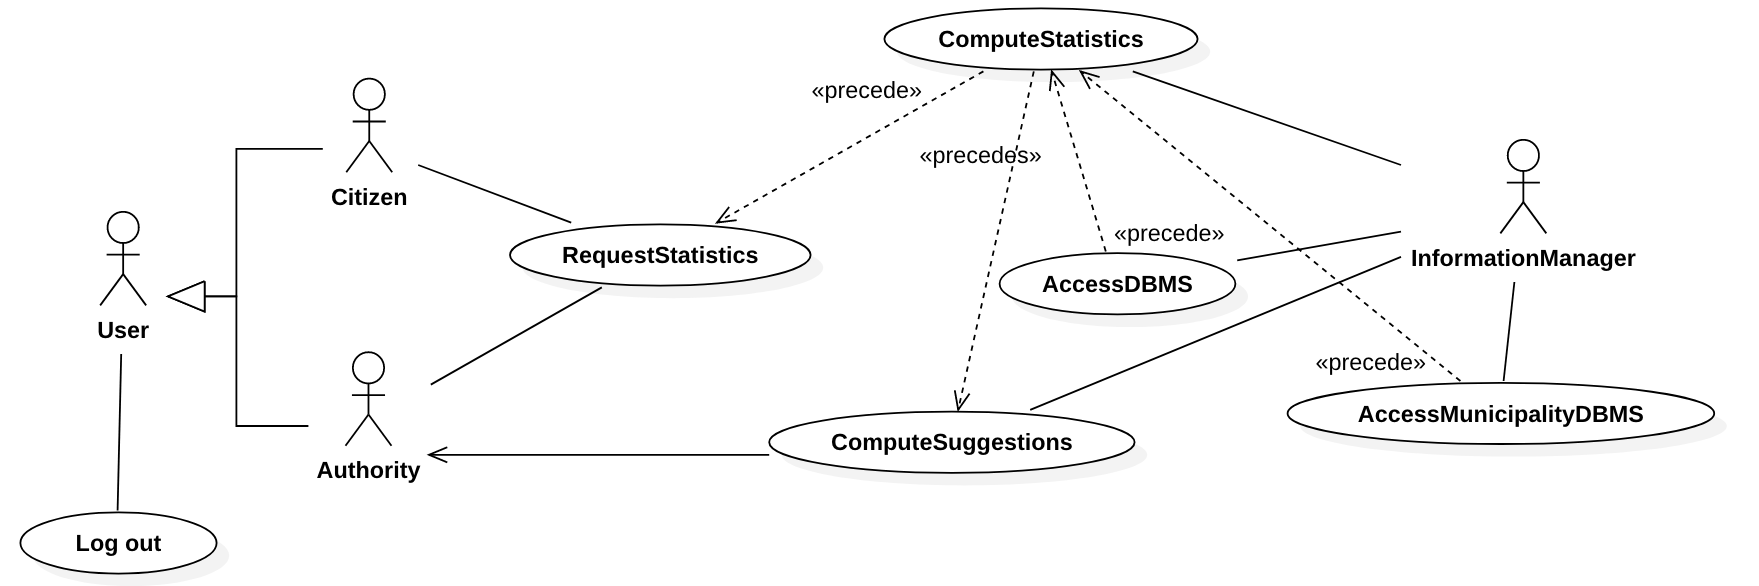
\includegraphics[width=\textwidth]{./img/UseCase3.png}
	\end{center}
	\caption{Information Manager use case.}
	\label{fig:UseCase3}
	\end{figure}
	\newpage
%%%%%%%%%%%%%%%%%%%%

\begin{center}
	\textbf{Compute Statistics}
\end{center}
\begin{tabularx}{\linewidth}{| l | X |}
	\hline
	\textbf{ID} & UC5\\
	
	\hline
	\textbf{Description} & A \textbf{\textit{User}} wants to see some statistics (e.g the safety of a certain area) and ask the \textbf{\textit{Information Manager}} about them.\\
	
	\hline
	\textbf{Actors} & \textbf{\textit{User}} and \textbf{\textit{Information Manager}}\\
	
	\hline
	\textbf{Preconditions} & The \textbf{\textit{Information Manager}} has already computed the statistics that the user intends to consult. At set times, the \textbf{\textit{Information Manager}} updates all the statistics due to possible new stored reports. \\
	
	\hline
	\textbf{Flow of Events} & \parbox{0.7\textwidth}{\begin{enumerate}
			\item The \textbf{\textit{User}} logs in to the application and taps on the \textit{Statistics} button.
			\item The \textbf{\textit{System}} displays a menu with all the possible statistic options to compute.
			\item The \textbf{\textit{User}} chooses the statistics in which he/she is interested in.
			
			\item The \textbf{\textit{Information Manager}} loads the statistics that the user selected and the application shows. 
			\begin{itemize}
				\item The application may use external services to show some statistics on a map.
				\item If the \textbf{\textit{User}} who requested to see the statistics is an Authority, the \textbf{\textit{Information Manager}} will also show him/her the latest safety suggestions (if available).
			\end{itemize}
			
	\end{enumerate}}\\
	
	\hline
	\textbf{Postconditions} & The \textbf{\textit{User}} sees the results of the statistics request.\\
	
	\hline
	\textbf{Exceptions} & \parbox{0.7\textwidth}{ \begin{enumerate}
			\item If the \textbf{\textit{Municipality}} doesn't allow the System access traffic ticket information, the \textbf{\textit{Information Manager}} can't retrieve this type of data and the The \textbf{\textit{User}} can't visualize the traffic tickets statistics. In this case, a message saying \textit{Statistic Unavailable} is shown to the The \textbf{\textit{User}}. The flow restart from point 3.  
		\end{enumerate}}\\
	
	\hline
	
\end{tabularx}
%%%%%%%%%%%%%%%%%%%%%%%%
\newpage
\subsection{Sequence Diagrams}
\begin{figure}[ht!]
	\begin{center}
	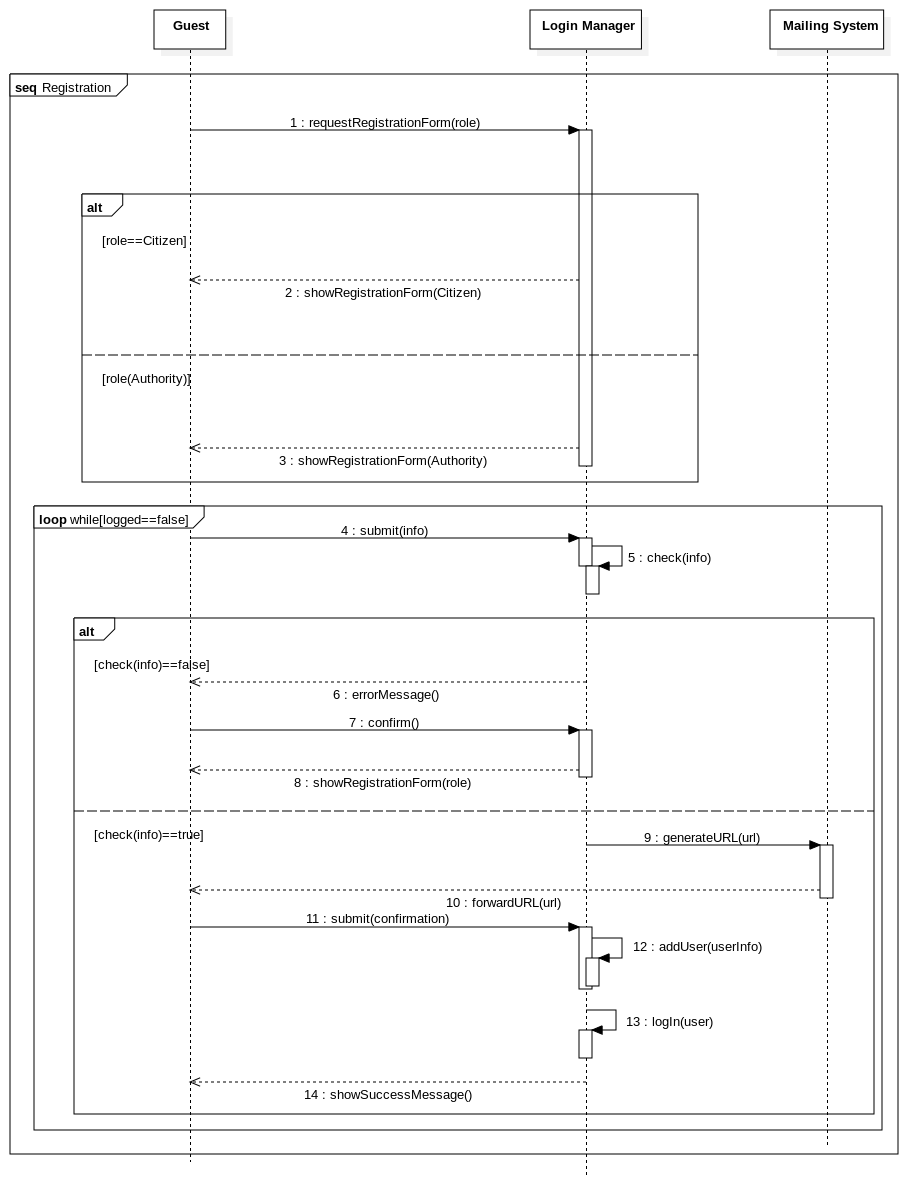
\includegraphics[width=\textwidth]{./img/RegistrationSd.png}
	\end{center}
	\caption{Sign up Sequence Diagram.}
	\label{fig:SequenceDiagram1}
	\end{figure}
\newpage
\begin{figure}[ht!]
\begin{center}
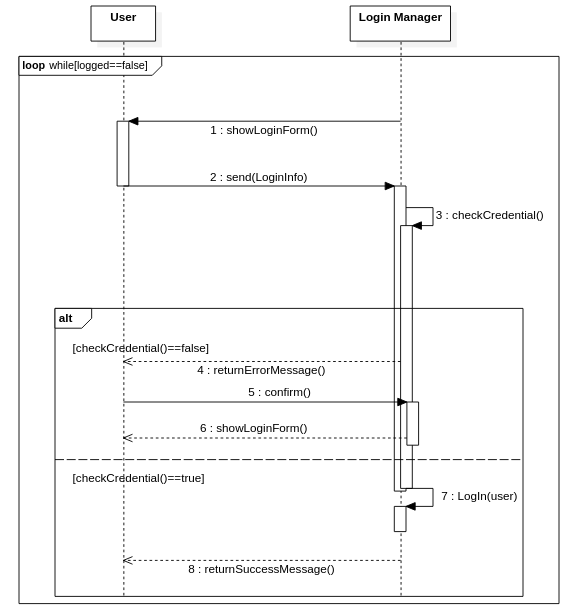
\includegraphics[width=\textwidth]{./img/LoginSD.png}
\end{center}
\caption{Login Sequence Diagram.}
\label{fig:SequenceDiagram2}
\end{figure}
\newpage
\begin{figure}[ht!]
\begin{center}
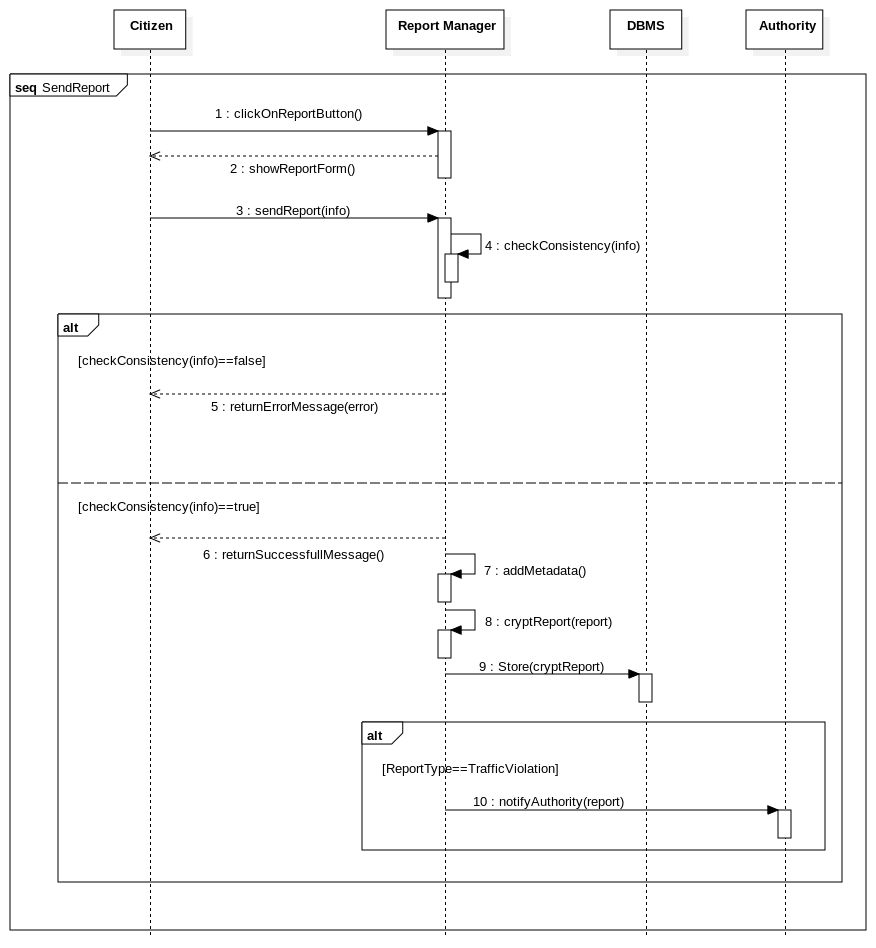
\includegraphics[width=\textwidth]{./img/SendReportSd.png}
\end{center}
\caption{Send Report, notify and Store report Sequence Diagram.}
\label{fig:SequenceDiagram3}
\end{figure}
\newpage
\begin{figure}[ht!]
\begin{center}
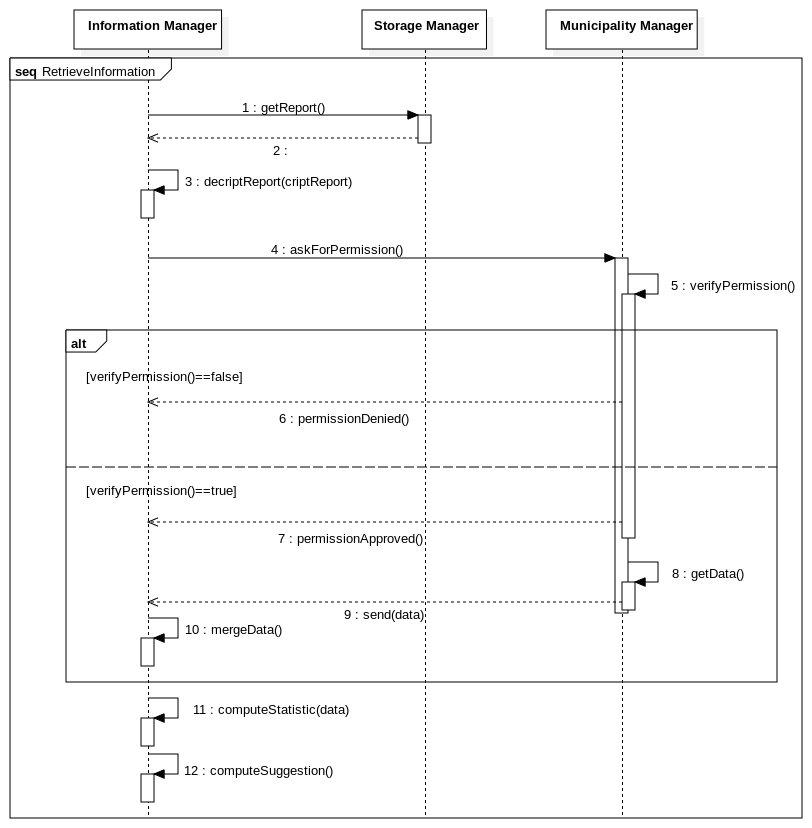
\includegraphics[width=\textwidth]{./img/RetrieveSd.png}
\end{center}
\caption{Retrieve Information Sequence Diagram.}
\label{fig:SequenceDiagram4}
\end{figure}

\newpage 

\subsection{Goals Mapping on Requirements and Assumptions}
%Intro
\begin{itemize}
	\item \textbf{{[G.1]} The System allows Users to access the functionalities of the application from different locations and devices.}
\begin{center}\large{\textit{Requirements}}\end{center}
	\begin{itemize}
		\item{[R.1]} 
		A visitor must be able to register. During the registration the System will ask to provide some credentials.
		\item {[R.2]} The System must check if the Guest credentials are valid:
	        \begin{itemize}
	            \item the email is in the right format.
	            \item the password has a minimum length.
	            \item the municipality, if it is an Authority.
	            \item the username is not already taken by another registered User.
	        \end{itemize}
		\item {[R.3]} The System must store all User data such as personal information and credentials.
		\item {[R.5]} 
		The System must allow the User to change username, but only if the
		new username is not already in use by another User, email, but only if the
		new email is in a correct format, and password, only if the new password is different from the precedent and respects the minimum length.
		\item {[R.6]} The System must send a confirmation email if username, email
		or password is changed (similarly to the registration process).
		\item {[R.7]} 
		The System must allow the User to change password if it has been forgotten,through the personal email.
	\end{itemize}
\begin{center}\large{\textit{Domain Assumptions}}\end{center}
	\begin{itemize}
		\item {[D.1]} The registration mail is assumed to be correctly recieved by the User.
	\end{itemize}
	\vspace{3mm}
	\textbf{\item {[G.2]} The System allows Guests to authenticate themselves either as Authority or Citizen.
		\begin{itemize}
			\item {[G.2.1]}The System offers different levels of visibility to different roles.
		\end{itemize}}
\begin{center}\large{\textit{Requirements}}\end{center}
    \begin{itemize}
		\item {[R.4]} The System must allow the User to log in using his/her personal credentials.
		\item {[R.13]} The System provides a recognition system of badge number.
    	\item {[R.15]} The System must allow the User to see its position in a map.
	\end{itemize}
	\vspace{3mm}
    \item \textbf{{[G.3]} The System allows the Citizens to document traffic violations and accidents to Authorities by compiling a Report.}
\begin{center}\large{\textit{Requirements}}\end{center}
	\begin{itemize}
		\item {[R.8]} The User must be allowed to create reports, specifying:
	        \begin{itemize}
	            \item The type of report (violation/accident).
	            \item The location of the violation/accident.
	            \item The date of the violation/accident.
	            \item The time of the violation/accident.
	            \item A picture of the violation/accident (not mandatory).
	        \end{itemize}
		\item {[R.9]} The System must check if the Report created by the User is correct.
		\item {[R.14]} 
		The System must allow the Citizen to consult the history of its personal reports.
	\end{itemize} 
	\vspace{3mm}
	\item \textbf{{[G.4]} The System stores the reports provided by the Citizens.
		\begin{itemize}
			\item {[G.4.1]} If the Citizen has not provided any information about the license plate, the System runs an algorithm to read it from the submitted picture.
		\end{itemize}}
\begin{center}\large{\textit{Requirements}}\end{center}
    \begin{itemize}
		\item {[R.10]}
		The System must notify the Authorities whenever a new Report involving their municipality is submitted. 
		\item {[R.20]}
		The System can use third part services to read the license plate from the pictures.
	\end{itemize}
\begin{center}\large{\textit{Domain Assumptions}}\end{center}
	\begin{itemize}
		\item {[D.2]} The System internal clock time used to provide notifications is correct.
		\item {[D.3]}
		 The Authorities notifications are assumed to be made only in case of parking violations. Indeed, if a little accident occurs there is no need to contact the Authorities. Instead if a dangerous accident happens it is better to call the Autorithies for a promptly intervention. The System uses accident report only to make statistics.
	\end{itemize}
	\vspace{3mm} 
	\item \textbf{{[G.5]} The System must allows Authorities to consult Reports.}
\begin{center}\large{\textit{Requirements}}\end{center}
	\begin{itemize}
		\item {[R.16]} The System notify a copy of a report about traffic violation to Authorities.
		\item {[R.17]} The System provides a list of the most recent reports submitted to the Authorities.
    	\item {[R.18]} The System provides an history of reports submitted to the Authorities.
	\end{itemize}
\begin{center}\large{\textit{Domain Assumptions}}\end{center}
	\begin{itemize}
		\item {[D.4]}
		The Authorities are assumed to  take measures when they are notified about a new report.
	\end{itemize} 
	\vspace{3mm}
	\item \textbf{{[G.6]} The System analyzes the stored information to build statistics.
	\begin{itemize}
		\item {[G.6.1]}If allowed by the Municiplaity, SafeStreets can cross their information about accidents with its own in order to improve the analysis.
	\end{itemize}}
\begin{center}\large{\textit{Requirements}}\end{center}
    \begin{itemize}
		\item {[R.11]}
		The System must provide two different level of visibility regarding the statistics. Only the Authorities can consult statistics with private data.
    	\item {[R.12]} The System must allow the User to consult the statistics.
    	\item {[R.19]} The System must interact with the Municipality to get the permission for using their data.
		\item {[R.21]} The System has to update the statistics periodically.
		\item {[R.24]} The System can cross the data coming from external DBMS \\with its own data.
	\end{itemize}
\begin{center}\large{\textit{Domain Assumptions}}\end{center}
	\begin{itemize}
		\item {[D.5]} After the first time, the System does not need to request the access to the Municipality's’ DBMS as long as the permission is still valid..
    	\item {[D.6]} The statistics and suggestions are assumed to be consulted by Authorities periodically, in order to provide a better service.
    	\item {[R.23]} The System must be able to acknowledge whether or not multiple istances of Reports are referred to the same infraction, even if protracted over time.
	\end{itemize}
	\vspace{3mm}    
	\item \textbf{{[G.7]} The System is able to detect unsafe areas.
		\begin{itemize}
			\item {[G.7.1]} The System can suggest possible interventions to the Authorities.
		\end{itemize}}
\begin{center}\large{\textit{Domain Assumptions}}\end{center}
	\begin{itemize}
		\item {[D.6]} The statistics and suggestions are assumed to be consult by Authorities periodically, in order to provide a better service. 
	\end{itemize}
	\vspace{3mm}
    \item \textbf{{[G.8]} If allowed by the Municiplaity, SafeStreets can access their information about issued tickets to build statistics and evaluate its effectiveness.
    \begin{itemize}
        \item {[G.8.1]} The System ensures that the chain of custody of the information coming from the Citizens is never broken.
	\end{itemize}}
\begin{center}\large{\textit{Requirements}}\end{center}
	\begin{itemize}
		\item {[R.22]} The System must provide protection of data using encryption.
	\end{itemize}
\begin{center}\large{\textit{Domain Assumptions}}\end{center}
	\begin{itemize}
        \item {[D.7]} Only specific component of the System is able to decrypt sensible data.
	\end{itemize}
	\vspace{3mm}
	\item \textbf{{[G.9]} The System allows the User to consult statistics
	\begin{itemize}
		\item {[G.9.1]} The System offers different levels of visibility to different roles.
	\end{itemize}}
\begin{center}\large{\textit{Requirements}}\end{center}
	\begin{itemize}
		\item {[R.12]} The System must allow the User to consult the statistics.
		\item {[R.21]} The System has to update the statistics periodically.
	\end{itemize}
\end{itemize}

\newpage

\section{Performance Requirements}
SafeStreets is an application who's main job is to compute statistics and show the results to its Users. The collection of the data and the computation of the statistics are operations carried out by two distinct modules (respectively the Report Manager and the Information Manager) which write and read the database independently and asynchronously. This design is thought to benefit the performances: in conditions of high traffic the Report Manager can store the recieved Reports into a buffer and export later into secondary memory, whereas the Information Manager can suspend the computation of statistics and present to the requesting Users older results previously computed.
\section{Design Constraint}
As already mentioned in Section \ref{constraints}, since the System is not designed to provide a function to generate official traffic tickets, we can only assume that the Authorities will handle the reported traffic violations properly. For this reason, the System is not aware of whether or not the violation is being handled, at least as long as a corresponding traffic ticket is generated by an Authority (and the System has the authorization to access such data). However, the System cannot distinguish a traffic ticket generated with the help of SafeStreets by one that is not.
\subsection{Standards Compliance}
\begin{itemize}
	\item \textbf{GDPR} with regard to the processing of the User's personal data.
	\item \textbf{Latitude and Longidute degrees} for all the information regarding locations.
\end{itemize}
\subsection{Hardware Limitations}
The application should be able to run, at least, under the following condi-
tions:
\begin{itemize}
	\item iOS or Android smartphone
	\item 3G connections at 2Mb/s
	\item 50 MB of space
	\item 2 GB of RAM
\end{itemize}
\newpage
\section{Software System Attribute}
This section will cover the non-functional requirements that might be used to evaluate the software performances. All of the covered requirements are part of the ISO/IEC 9126-1:2001 (see Section \ref{docs}).
\subsection{Reliability}
The System (and all its components) should guarantees a 99\% of reliability. In order to guarantee the continuity of the service, it must be ensured that the System is fault tolerant.
\subsection{Availability}
The System must guarantee an high availability, indeed it has to offer a continuous service 24/7. 
\subsection{Security} \label{sec:security}
User credentials and data will be stored in a DBMS that should guarantee an high level of security. To reach this goal the passwords stored in the DBMS are salted and hashed, in this way a sequence of generic characters of any length is concatenated to the password, hashed it all and stored in the DBMS.
Hash is used also to stored the report so that the informations cannot be altered by anyone. So as soon as a report arrives to the Report Manager, the hash of the report is computed, encrypted to form a digital signature and then it is stored. In this way we create a snapshot of the report ensuring the identity, authenticity and non-tampered state of the informations.
As mentioned before, the System uses HTTP over SSL protocol (HTTPS) to comunicate with all the services in order to guarantee privacy and protection of the exchanged informations.
\newline
If someone break into the OCR tool or the Map service, the System is not responsible in case of damage, due to the fact that its functionalities are provided by third-part services.  
\subsection{Maintainability}
The System will have a modular architecture: Report Manager, Login Manager and Information Manager are designed to work separately in an asynchronous way, thus the maintenance process will be sped up in case of failure of one module.
\subsection{Portability}
SafeStreets is developed in terms of a native application on Android and iOS.
\end{document}